\chapter{The Problem and its Background}

As it was shown in the introduction, this work pretends to prove several VAD and SPP methods for the multichannel Wiener filter algorithm for speech enhancement. In this chapter will be explained how this filter works and why it is important to test the performance of the SPP block.


\section{Signal Model}

To maintain mathematical coherence during the document, the signal model will always be as it follows:

The microphone signals will be denoted as:

$$Y_m(k,n),l=1,...,M$$

Where $k$ is the frequency bin index, $n$ is the frame index and $M$ is the number of microphones. So, the input signals are given by:

$$Y_m(k,n)=X_m(k,n)+V_m(k,n)$$

Where $X_m$ and $V_m$ are the target signal and the uncorrelated noise components. The goal is to remove the unwanted noise and preserve the target signal, this can be done by using a filter set $\textbf{w}(k,n)$ to obtain:

$$Z(k,n)=\textbf{w}^H(k,n)\textbf{y}(k,n)$$



Where $Z$ is the output signal and $\textbf{y}(k,n)$ is a vector given as:

$$\textbf{y}(k,n) = [Y_1(k,n), Y_2(k,n),...,Y_M(k,n)]^T $$
$$\textbf{y}(k,n)= \textbf{x}(k,n)+\textbf{v}(k,n)$$

The correlation matrices of noisy speech, clean speech and noise are defined as:

$$\textbf{R}_y=E\{\textbf{yy}^H\}  	\in \mathds{C}^{M\times M}$$
$$\textbf{R}_x=E\{\textbf{xx}^H\}	\in \mathds{C}^{M\times M}$$
$$\textbf{R}_v=E\{\textbf{vv}^H\}	\in \mathds{C}^{M\times M}$$



\section{Multi-Channel Wiener Filter}

Many of the real time implementations of the multichannel Wiener filter (MWF) have estimation problems caused mainly for using a voice activity detector (VAD), which may fail in adverse environments and the use of second order clean speech statistics, which usually causes overestimation errors. In this document it will be described the algorithm proposed in \cite{Yong2013}, first using the hard VAD and then using a SPP. Also, in order to have a better performance it will be chosen one of the input signals from the microphone array and will be filtered by a single channel algorithm and this new signal will be used as reference (the complete block diagram is shown in figure \ref{fig:diagMWF}). Finally it will be shown the objective tests that were applied to this algorithm in order to show a comparison with other  methods.

\begin{figure}[!ht]
  \centering
	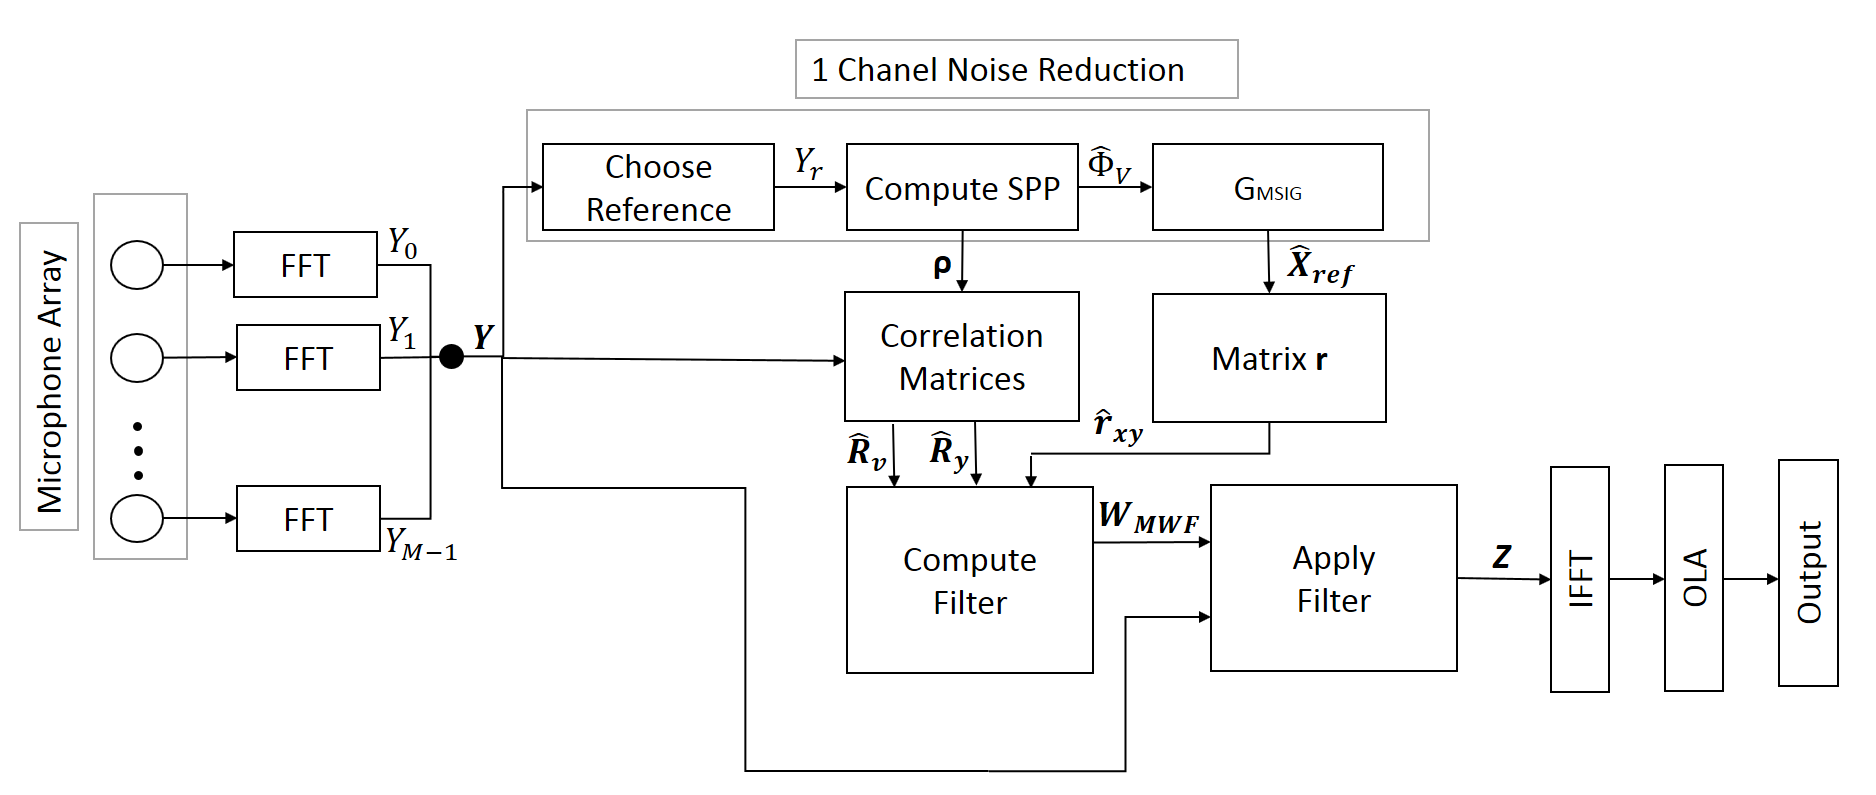
\includegraphics[width=150mm]{Kap2/diagMWF}
	\caption{Block diagram for multichannel Wiener filter.}
	\label{fig:diagMWF}
\end{figure}

\subsection{Filter Formulation}

It is expected to estimate the speech signal based on an minimum mean square error criterion as:

\begin{equation}
\textbf{w}_{MWF}=arg min_w E\{|X_{ref}-\textbf{w}^H \textbf{y}|^2 \}
\label{criteria}
\end{equation}


If it is taken the assumption of uncorrelation between speech and noise, it is possible to modify the criterion of the MWF as:

$$\textbf{w}_{MWF}=arg min_w E\{|X_{ref}-\textbf{w}^H \textbf{x}|^2 \}+\mu E\{|X_{ref}-\textbf{w}^H \textbf{v}|^2 \}$$

A larger $\mu$ value here indicates more residual noise reduction at the expense of higher speech distortion. The solution of $MWF_\mu$ can then be obtained as:

\begin{equation}
\textbf{w}_{{MWF}_\mu} = [\textbf{R}_x+\mu \textbf{R}_v]^{-1}\textbf{R}_x\textbf{e}_{ref}
\label{wiener}
\end{equation}

Where $\textbf{e}_{ref}=[0...0 1 0...0]^T$ is a M-element zero vector with the unity corresponds to the $m^{th}$ element of the microphones. 


In first place, the update of the correlation matrices can be done like:

\begin{equation}
\mathcal{H}_0 : \left\{
\begin{array}{c l}
   \hat{\textbf{R}}_v[n]=(1-\alpha_v)\hat{\textbf{R}}_v[n-1]+\alpha_v\textbf{y}[n]\textbf{y}^H[n] \\
  \hat{\textbf{R}}_y[n]= \hat{\textbf{R}}_y[n-1]
\end{array}
\right.
\end{equation}

\begin{equation}
\mathcal{H}_1 : \left\{
\begin{array}{c l}
   \hat{\textbf{R}}_y[n]=(1-\alpha_y)\hat{\textbf{R}}_y[n-1]+\alpha_y\textbf{y}[n]\textbf{y}^H[n] \\
  \hat{\textbf{R}}_v[n]= \hat{\textbf{R}}_v[n-1]
\end{array}
\right.
\end{equation}

Where  $\mathcal{H}_0$  and  $\mathcal{H}_1$ denote the periods of absence and presence of speech. This periods are determined by the use of a VAD algorithm. The choice of the smoothing factors  $\alpha$ must be done carefully taking care if the  degree of stationarity of speech and noise signals.

In equation \eqref{wiener} it is needed an estimation of $\textbf{R}_x$ which could be obtained form $\textbf{R}_y-\textbf{R}_v$, but this estimation might have some errors caused by the complex valued matrices, which will lead to a bad estimation.  This estimation could be improved by obtaining a pre-determined $R_x$ estimate  with a calibration sequence, or by implementing a mathematical model, these methods rely on the a priori information, which makes them less stable and difficult to use for final users. 

\subsection{Formulation of {$MWF_\lambda$}  and Estimation of Correlation Matrices}

To minimize the error from equation \eqref{criteria}, another criterion to minimize the noise power is proposed. For this, one weighed sum can be find as:

$$\textbf{w}_{MWF_\lambda}=argmin_w(1-\lambda)E\{|X_{ref}-\textbf{w}^H\textbf{y}|^2\}+\lambda(E\{|\textbf{w}^H\textbf{v}|^2\})$$

Where $\lambda$ is a weighting value between 0 and 1, this solution is given by:

\begin{equation}
\textbf{w}_{MWF_\lambda}=[(1-\lambda)\textbf{R}_y+\textbf{R}_v]^{-1}(1-\lambda)\textbf{r}_{yx}
\label{mwfl}
\end{equation}


$$\lambda=1-\rho$$
where $\textbf{r}_{yx}=E\{\textbf{y}X^*_{ref}\}$.   Using this consideration, it is avoided the estimation of $\textbf{R}_x$ and the value of $\lambda$ can be set as $1-\rho$ where $\rho$ is the SPP of the signal. Also,  it is proposed to avoid the decision by the VAD to estimate the correlation matrices and to use instead a modified SPP ($\rho$) with which the matrices can be estimated as:




\begin{equation}
\hat{\textbf{R}}_v[n]=(1-\tilde{\alpha}_v[n])\hat{\textbf{R}}_v[n-1]+\tilde{\alpha}_v[n]\textbf{y}[n]\textbf{y}^H[n] 
\label{corrv}
\end{equation}

\begin{equation}
\hat{\textbf{R}}_y[n]=(1-\tilde{\alpha}_y[n])\hat{\textbf{R}}_y[n-1]+\tilde{\alpha}_y[n]\textbf{y}[n]\textbf{y}^H[n]
\label{corry}
\end{equation}


Where $\tilde{\alpha}_v$ and $\tilde{\alpha}_y$  are given by:

$$\tilde{\alpha}_v=\alpha_v(1-\rho)$$ and

$$\tilde{\alpha}_y=\alpha_y\rho$$

Where $\alpha_v$ and $\alpha_y$ are the fixed smoothing factors for noise and noisy correlation matrices and $\rho$ is the value of the speech presence probability. 


\subsubsection{Smoothing the filter}

In the first implementation, as proposed in \cite{Yong2013}, the output signal tends to have musical noises. To solve this, it is proposed to do a smoothing process over the whole filter $\textbf{W}_{MWF_\lambda}$ as:

\begin{equation}
 \textbf{W}_{MWF_\lambda}(k,n)= \alpha_w\textbf{W}_{MWF_\lambda}(k,n-1)+(1-\alpha_w) [(1-\lambda)\textbf{R}_y+\textbf{R}_v]^{-1}(1-\lambda)\textbf{r}_{yx}
\label{mwfeq}
\end{equation}


Which leads to an important musical noise reduction.

\subsubsection{Single-Channel Reference}

From equation \eqref{mwfl}, we can see that this method needs the estimate of the speech reference $X_{ref}$, to achieve this, it is proposed to estimate $X_{ref}$ by using a single-channel speech enhancement method and to use one microphone as a reference. With this, it is possible to define: $$\tilde{\textbf{r}}_{yx}=\textbf{y}G(X^*_{ref}+V^*_r)$$

Where $X_{ref}=H_{ref}S$, in which $H_{ref}$ is the acoustic transfer function of the target speech signal $S$, at the reference channel. In this equation $G$ is a spectral weighting gain function, which involves the computation of the \textit{a posteriori }and \textit{a priori} SNR estimates. Also, to avoid musical noise, it is proposed to update recursively $\hat{\textbf{r}}_{yx}(n)$ as:

\begin{equation}
\hat{\textbf{r}}_{yx}(n)=(1-\alpha_x)\hat{\textbf{r}}_{yx}(n-1)+\alpha_x\textbf{y}(n)\hat{X}^*_{ref}(n)
\label{requ}
\end{equation}


Where $\alpha_x$ is the smoothing  factor for target speech signal, and $\hat{X}_{ref} = G(X_{ref}+V_r)$  indicates the clean speech estimate from the reference microphone.  This estimate  can be done with any of the existent speech enhancement methods, but it is recommended to use one in which the  speech distortion can be controlled and set it as small as possible. In this case it will be used the one found in \cite{Yong2013OptimizationEnhancement}. This method works as follows:   

\subsubsection{Sigmoid function with \textit{a priori} SNR}



In order to find $\hat{X}_{ref}$ it is needed to chose one of the channels as a reference, in our case the input  of the closest microphone to the source can be chosen. This signal must be filtered with one method of speech enhancement. 


In \cite{Yong2013OptimizationEnhancement} it is proposed to use a gain function which can be easily controlled and that has a flexible shape.   In this case we use the modified sigmoid gain function:

\begin{equation}
G_{MSIG}(k,n)=\frac{1-exp[-a_1 \hat{\xi}(k,n)]}{1+exp[-a_1 \hat{\xi}(k,n)]}*\frac{1}{1+exp(-a_2 [\hat{\xi}(k,n)-c])}
\label{gainSig}
\end{equation}

Where $\xi$ is the  \textit{a priori} SNR  defined as 
$$\xi(k,n)=\frac{\Phi_x(k,n)}{\Phi_v(k,n)}$$

Which can be estimated as a function of the \textit{a posteriori} SNR and an instantaneous \textit{a priori} SNR, the \textit{a posteriori} SNR and applying a recursive smoothing procedure:

$$\xi_{inst}(k,n)=max\{\gamma(k,n)-1,0\}$$

using the fact that $X(k,n-1)=G_{MSIG}(k,n)Y(k,n-1)$:

$$\hat{\xi}(k,n)=\alpha_{SNR}G_{MSIG}^2(k,n-1)\gamma(k,n-1)+(1-\alpha_{SNR})\xi_{inst}(k,n) $$
The variance in the\textit{ a priori} SNR estimate can lead to audible musical noise due to the higher sensitivity to changes. In order to reduce such musical noise, a first order recursive smoothing procedure, as shown in \cite{Yong2011OnEnhancement}, can be applied in the \textit{a posteriori }SNR estimation:

$$\bar{\gamma}(k,n)=\frac{\Phi_y(k,n)}{\hat{\Phi}_v(k,n)}$$
With:

$$\Phi_y(k,n)=\alpha_{y'}\Phi_y(k,n-1)+(1-\alpha_{y'})|Y(k,n)|^2$$



The resulting function of equation \eqref{gainSig}  can have different shapes as shown in \ref{fig:sigm} according to the choice of the constants $a_1$, $a_2$ and $c$, for this implementation the values were chosen as function MSIG-fix3:

$$a_1=15$$
$$a_2     = 0.6351$$
$$c       = 0.2243$$
\begin{figure}[!ht]
  \centering
	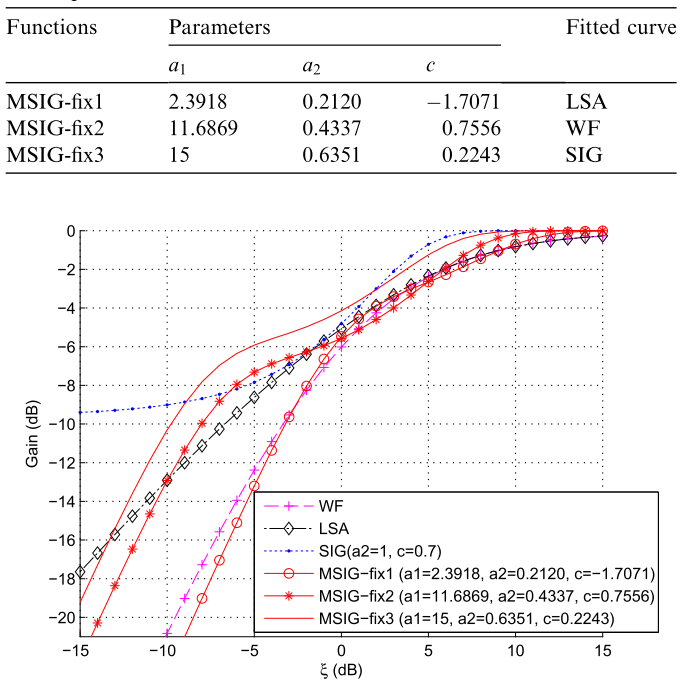
\includegraphics[width=110mm]{Kap2/sigm}
	\caption{Different shapes of the gain function, taken from \cite{Yong2013OptimizationEnhancement}.}
	\label{fig:sigm}
\end{figure}



\section{Speech Presence Probability}

Several authors have made important research on SPP methods. 

All real time audio processing algorithms are implemented with short time Fourier transformations (STFT). The speech presence probability method, has as output a vector of the same size than each frame vector, each element of this vector is a real number with values from 0 to 1 which denote the probability of finding voice in each frequency bin. In this case 0 is the lowest probability of finding voice and 1 is the highest. In the figure \ref{fig:spectro} it is shown the spectrogram of a clean female voice signal and in figure \ref{fig:SPP} it is shown all the SPP vectors of this signal. 

\begin{figure}[!ht]
  \centering
	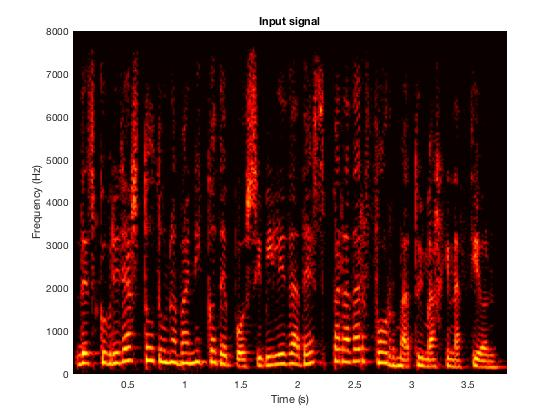
\includegraphics[width=100mm]{Kap2/spectro}
	\caption{Spectrogram of a clean voice audio file.}
	\label{fig:spectro}
\end{figure}

It is possible to see that, in an ideal SPP (absence of noise), the output has the value of 1 in each bin where there is presence of speech in the signal. Note that in an ideal case all speech presence values should be 1 and this does not depend on the magnitude of the voice energy in the signal, following the same logic, in silent segments or nose segments, the values should be 0. 

\begin{figure}[!ht]
  \centering
	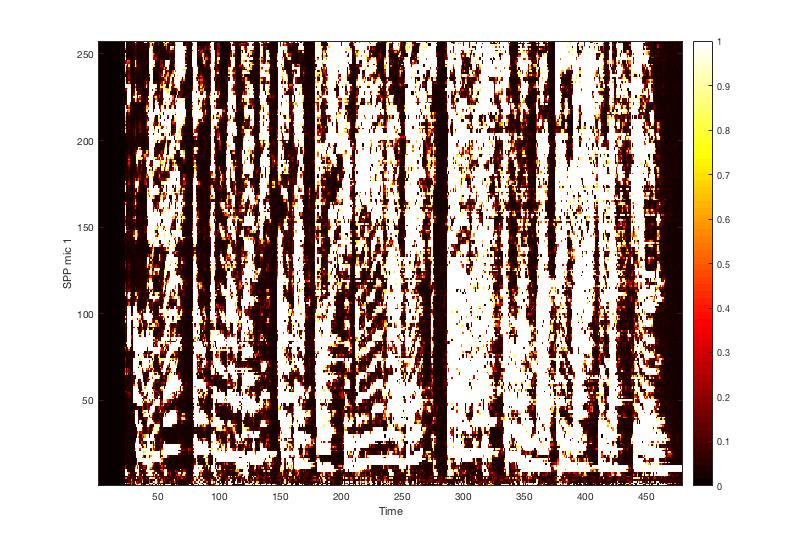
\includegraphics[width=100mm]{Kap2/SPP}
	\caption{Speech presence probability of a clean voice audio file.}
	\label{fig:SPP}
\end{figure}

In this project, different algorithms for finding the SPP will be tested under different SNR conditions. For testing this, the SNR of the output of the MWF will be compared for each SPP algorithm.

